\documentclass[sokoban_generation_thesis.tex]{subfiles}
Generowanie proceduralne to~tworzenie zawartości przy użyciu algorytmów. Zamiast tworzyć zawartość ręcznie, można to~zadanie zlecić wyspecjalizowanym metodom. Wykorzystanie komputerów do~generowania proceduralnego może przynieść więcej treści o~wyższej jakości niż ludzka kreacja manualna, dlatego w~dobie dynamicznego rozwoju technologii jest to~istotne zagadnienie. Wśród licznych przykładów wykorzystania generowania proceduralnego warto wymienić oprogramowanie \textit{Massive} \cite{massive_gen}, które generowało tłumy liczące setki tysięcy postaci w~bitwach z~filmowej trylogii \textit{Władcy Pierścieni} czy też \textit{Terragen} \cite{terragen}, przy wykorzystaniu którego artyści i~fotografowie dodają głębi przedstawianym krajobrazom.

Przemysł komputerowych gier wideo jest dynamicznie rozwijającą się gałęzią gospodarki. Wartość rynku gier, jako jednego z~najmłodszych przemysłów kreatywnych, wyróżnia się monotonicznym tempem wzrostu \cite{game_industry_creative}. W~roku $2019$ wyceniało się rynek gier na~ponad $150$ miliardów dolarów, a~wzrost jego wartości w~latach $2018-2022$ szacuje się na~$27\%$ \cite{game_industry_creative}. Z~tegorocznych analiz wynika, że~branża gier przynosi więcej zysków niż filmowa i~muzyczna razem wzięte \cite{e3_game_industry}. Reasumując, aktualna sytuacja jednoznacznie wskazuje na~to, że~ten dział branży kreatywnej jest w~rozkwicie.

\section{Proceduralne generowanie zawartości w~grach}
Podczas tworzenia gier, zatrudniani są~ludzie odpowiedzialni za~tworzenie grafik, animacji czy projektowania poziomów. Zamiast tego, można posiłkować się odpowiednimi technikami do~wygenerowania potrzebnego rodzaju zawartości.

Mówi się o~zastosowaniu generowania proceduralnego w~grach różnych gatunków. Przyjmuje się, że~jest to~technika powszechnie stosowana, która została zapoczątkowana w~roku 1978, wraz z~wydaniem \textit{Beneath Apple Manor} \cite{pcgrl_scanning}. W~tej produkcji zadaniem gracza jest sukcesywne przemierzanie kolejnych pokojów podziemnego świata, pokonując napotkanych na~swojej drodze wrogów. Twórcy \textit{Beneath Apple Manor} stworzyli algorytm generujący losowe pokoje, złożone z~losowych kombinacji wrogów. Takie rozwiązanie powoduje, że~każda rozgrywka będzie inna, tym samym stawiając przed graczem różne wyzwania.

Koncept proceduralnego generowania zawartości jest odciążeniem twórców gier. Coraz powszechniejsze staje się wykorzystywanie technik uczenia maszynowego w~tym celu, co~wykazano w~p.~\ref{subs:pcgrl_examples}. Istnieją jednak pewne obostrzenia z~tym związane, na~przykład czasowe. Techniki uczenia maszynowego najczęściej mają charakter iteracyjny i~wymagają dużej liczby iteracji w~celu osiągnięcia zadowalających wyników. Wobec tego, nieakceptowalne jest użycie tego rodzaju algorytmów w~czasie rzeczywistym w~grach. Zamiast tego, dokonuje się selekcji i~systematyzacji wygenerowanej zawartości i~dostarcza się ją~wraz z~grą \cite{deep_learning_pcgrl}.

\subsection{Przykłady}\label{subs:pcgrl_examples}
Interesującym zastosowaniem uczenia maszynowego w~generowaniu proceduralnym jest gra \textit{Galactic Arms Race} \cite{galactic_arms_race} wydana w~2014 roku przez \textit{Evolutionary Games}. Twórcy posiłkowali się autorskim algorytmem genetycznym, tworząc różne konfiguracje pocisków statków kosmicznych, takich jak na~rys.~\ref{rys:galactic_arms_race}. Algorytm \textit{cgNEAT} \cite{galactic_arms_race} ewoluuje, mając na~uwadze preferencje użytkownika, które są~określane na~bieżąco podczas rozgrywki. Oznacza to, że~twórcy nie musieli kreować działania i~graficznych aspektów pocisków -- ta~zawartość była tworzona przez algorytm.

\begin{figure}[H]
	\centering
	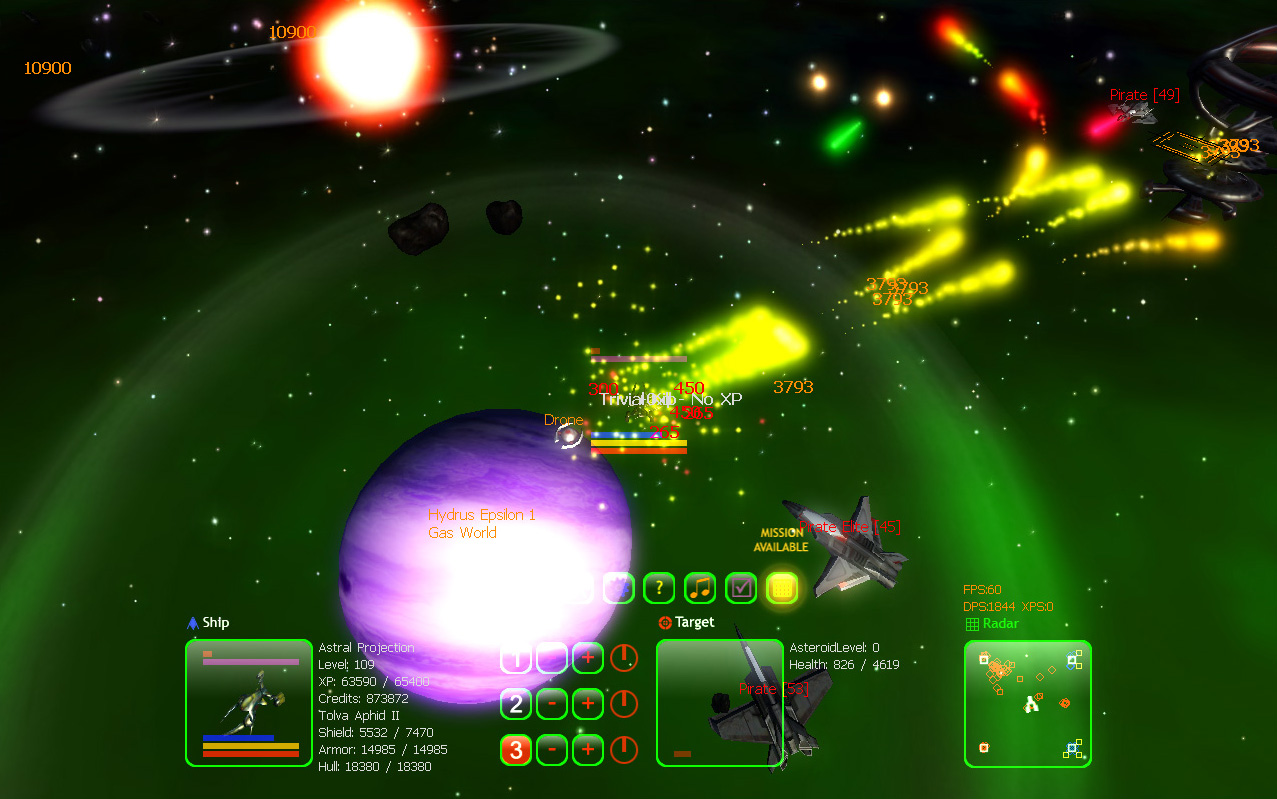
\includegraphics[width=0.8\textwidth]{galactic_arms_race}
	\caption{Zrzut ekranu z~gry \textit{Galactic Arms Race}, \\źródło: http://indiedb.com}
	\label{rys:galactic_arms_race}
\end{figure}

W grze \textit{Spelunky} zadaniem gracza jest przemierzanie kolejnych poziomów, co~wymaga zręczności i~szybkiego podejmowania decyzji. Twórcy \textit{Spelunky} zdecydowali się na~rozwiązanie hybrydowe w~kontekście generowania poziomów \cite{spelunky_gen}. Algorytm jest heurystyką, która działa w~oparciu o~podział poziomu na~$16$ części, jak na~rys.~\ref{rys:spelunky_gen}. Każda z~nich jest tworzona na~podstawie szablonu (ang.~\textit{template}), których zbiór został stworzy przez projektantów. Algorytm poprawia tak stworzony poziom, dodając element losowości i~zapewniając, że~istnieje ścieżka od~wejścia do~wyjścia z~poziomu.

Generowanie proceduralne nie jest techniką stosowaną wyłącznie w~nowych grach. Autorzy~\cite{mario_gan} wykorzystali generatywne sieci współzawodniczące (ang.~\textit{Generative Adversarial Networks}) do~tworzenia nowych poziomów w~kultowej grze \textit{Super Mario Bros.}, pochodzącej z~$1983$ roku.

\begin{figure}[H]
	\centering
	\begin{subfigure}[b]{0.43\textwidth}
		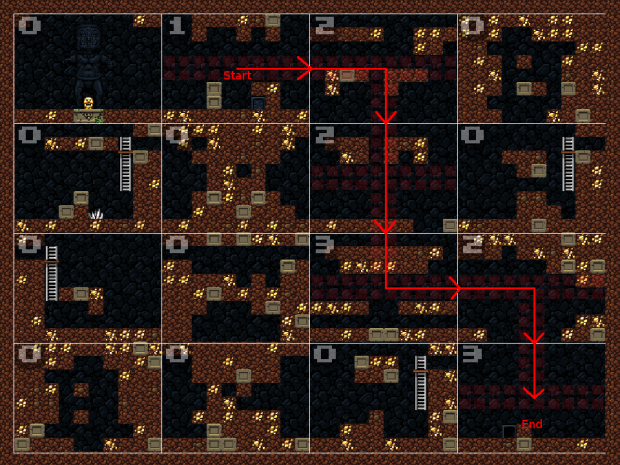
\includegraphics[height=5cm]{spelunky_gen}
		\caption{Poziom w~\textit{Spelunky}}
		\label{rys:spelunky_gen}
	\end{subfigure}
	\hspace{0.1\textwidth}
	\begin{subfigure}[b]{0.35\textwidth}
		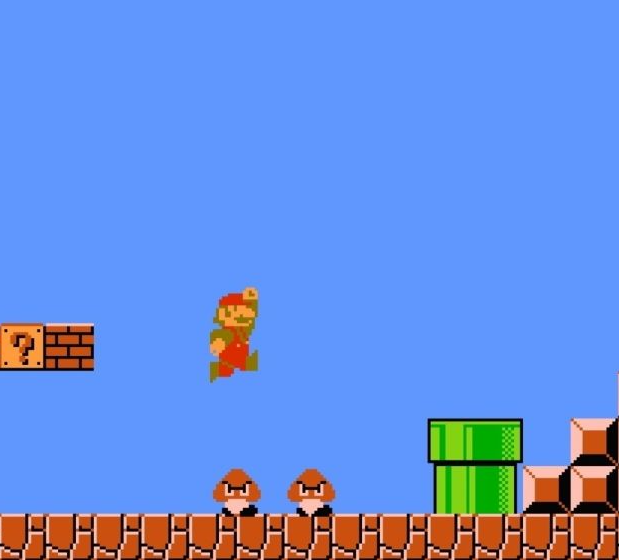
\includegraphics[height=5cm]{mario_level}
		\caption{Poziom w~\textit{Super Mario Bros.}}
		\label{rys:mario_level}
	\end{subfigure}
	\caption{Poziomy w~grach korzystających \\z generowania proceduralnego, źródła: \cite{spelunky_gen}, \cite{mario_gan}}
\end{figure}


Powszechnym podejściem w~generowaniu proceduralnym są~algorytmy generowania szumu gradientowego. Szczególnie często wykorzystuje się takie rozwiązania w~grach z~gatunku \textit{sandbox}, które przedstawiają graczom otwarty świat, nie narzucając sposobów jego eksploracji i~pozostawiając dowolność w~kwestii interakcji z~jego elementami. Gry takie jak \textit{Terraria} czy \textit{Minecraft}, tworzą dla graczy potencjalnie nieskończone światy dwu- lub trójwymiarowe.


\section{Sokoban} \label{subs:sokoban_intro}
\textit{Sokoban} jest grą logiczną, rozgrywaną na~planszy złożonej z~kwadratów. Celem gracza jest przesunięcie wszystkich pudeł  w~wyznaczone kwadraty docelowe, tak jak na~rysunku \ref{rys:board_rules_final}. Zasady gry nie zakładają przypisania pudeł do~pól docelowych -- każde pudło może trafić w~każde pole docelowe, o~ile zostanie to~wykonane zgodnie z~pozostałymi zasadami. 

Istnieje ujednolicony format zapisu poziomów do~formy tekstowej. Każde z~$7$ możliwych pól zamieniane jest na~odpowiedni znak, zgodnie z~tab.~\ref{tab:sokoban_format}.

\begin{table}[h!]
	\smallskip
	\centering
	\caption{Format zapisu plansz}
	\label{tab:sokoban_format}
	\begin{tabular}{|l|l|}
		\hline
		\textbf{Pole} & \textbf{Znak}\\ \hline
		Ściana & \# \\
		Gracz & @ \\
		Gracz na~polu docelowym & + \\
		Pudło & \$ \\
		Pudło na~polu docelowym & * \\
		Pole docelowe & .~\\
		Puste pole &  \\
		\hline
	\end{tabular}
\end{table}

Przykładowo, zaczynając z~planszą jak na~rys.~\ref{rys:board_rules_init}, gracz musi wykonać co~najmniej $8$ ruchów, w~tym $4$~pchnięcia pudeł. Jednak istnieje też rozwiązanie tej planszy, wykorzystujące $12$ ruchów, w~tym $2$ pchnięcia. Różne implementacje gry uznają liczbę ruchów albo liczbę pchnięć jako ocenę rozwiązania.

\begin{figure}[H]
	\centering
	\begin{subfigure}[b]{0.3\textwidth}
		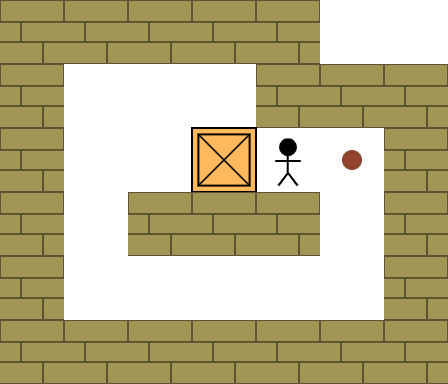
\includegraphics[width=\textwidth]{board_rules_init}
		\caption{Plansza początkowa}
		\label{rys:board_rules_init}
	\end{subfigure}
	\hspace{0.2\textwidth}
	\begin{subfigure}[b]{0.3\textwidth}
		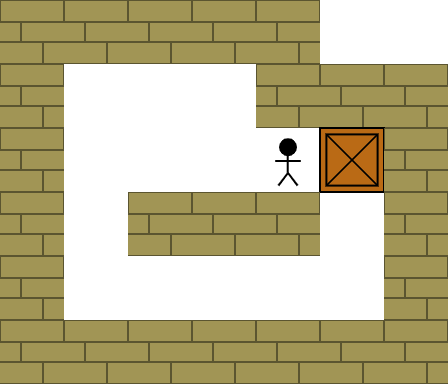
\includegraphics[width=\textwidth]{board_rules_final}
		\caption{Plansza końcowa}
		\label{rys:board_rules_final}
	\end{subfigure}
	\caption{Przykładowa plansza \textit{Sokoban}}
\end{figure}

Oryginalnie \textit{Sokoban} jest grą wideo autorstwa Hiroyuki Imabayashi, wydaną w~1982 roku na~platformę PC-88. Od~tamtego czasu koncepcja gry jest rozwijana i~implementowana w~innych grach, takich jak \textit{Pokémon Emerald} czy \textit{Grand Theft Auto: San Andreas}. Ponadto, użytkownicy tworzą coraz bardziej skomplikowane plansze, czego dowodem są~zbiory wymienione w~tab.~\ref{tab:sokoban_datasets}.

\begin{table}[h!]
	\smallskip
	\centering
	\caption{Zbiory plansz Sokoban, źródło: \cite{sok_wiki}}
	\label{tab:sokoban_datasets}
	\begin{tabular}{|l|l|}
		\hline
		\textbf{Nazwa zbioru} & \textbf{Liczba poziomów}\\ \hline
		Sven & 1911 \\
		Sasquatch I-VII & 350 \\
		Sokoban Perfect & 306 \\
		Sokoban Revenge & 306 \\
		Aymeric & 282 \\
		SokHard & 163 \\
		\hline
	\end{tabular}
\end{table}



\subsection{Rozwiązanie} \label{subs:solving_sokoban}
Problem podania rozwiązania czy choćby ustalenia, czy zadana plansza \textit{Sokoban} jest rozwiązywalna, jest problemem \textit{PSPACE}-zupełnym \cite{sokoban_pspace}. Problemy \textit{PSPACE}-zupełne to~grupa problemów, które mogą zostać rozwiązane przy użyciu maszyny Turinga, wykorzystując wielomianową ilość pamięci, ale nie są~problemami NP.

Drzewo decyzyjne odpowiadające rozgrywce, mimo swojego niskiego współczynnika rozgałęzienia (ang.~\textit{braching factor}), jest wysokie. W~przypadku rozwiązywania planszy \textit{Sokoban}, omawiany współczynnik wynosi co~najwyżej cztery, ponieważ w~każdej sytuacji gracz może dokonać ruchu w~jednym z~czterech kierunków. 

W związku z~tym, powstają heurystyczne \textit{solvery}, które potrafią rozwiązywać plansze \textit{Sokoban} w~czasie wielomianowym \cite{sok_wiki}. Mimo to, nie powstał jeszcze \textit{solver}, który rozwiązywałby poprawnie wszystkie plansze z~badanego zbioru \cite{sok_wiki}.

Problem rozwiązania planszy \textit{Sokoban} jest powiązany z~wieloma metodami generowania plansz. Metody generujące, które nie opierają swojego działania na~zasymulowaniu rozgrywki, potrzebują na~różnych etapach swojego działania weryfikować, czy aktualnie tworzona plansza jest rozwiązywalna. Jako że~sprawdzenie tego w~sposób dokładny nie jest możliwe czasowo, w~tym celu również wykorzystywane są~heurystyczne \textit{solvery}.
